\section{Conditional entropy calculation}
\begin{itemize}
\label{sectioncondcalc}
\item
Now for the Conditional Entropy calculation we will take a state created experimentally at \cite{gomez2019experimental}. It is a general form of entangled photons looking like:
\begin{equation}
|\psi(\theta)\rangle=\cos \theta|00\rangle+\sin \theta |11\rangle
\label{condentpsi}
\end{equation}
with $0< \theta< \pi /2$ to ensure entanglement and avoid ill-defined calculations with infinities.
Now we have to calculate both the von Neumann entropy of the whole state, and the von Neumann entropy for the partially traced sub-state that we choose as the conditional. All these, according to the \defref{defcondin}.
From \eqref{condentpsi} we deduce its density matrix:
\begin{equation}
\label{sigmastate}
\sigma^{AB}=\left(
\begin{array}{cccc}
 \cos ^2 \theta & 0 & 0 & \cos \theta \sin \theta \\
 0 & 0 & 0 & 0 \\
 0 & 0 & 0 & 0 \\
 \cos \theta \sin \theta & 0 & 0 & \sin ^2 \theta  \\
\end{array}
\right)
\end{equation}
We find the eigenvalues and eigenvectors of $\sigma$:

\begin{equation}
\lambda_1=1,\:  \lambda_2=0,\:  \lambda_3=0,\:  \lambda_4=0, 
\end{equation}
\begin{equation}
v_1=\left(
\begin{array}{c}
 \cot \theta \\
 0\\
 0\\
 1 \\
\end{array}
\right),
\:  v_2=\left(
\begin{array}{c}
 -\tan \theta \\
 0\\
 0\\
 1 \\
\end{array}
\right),
\:  v_3= \left(
\begin{array}{c}
 0 \\
 0\\
 1\\
 0 \\
\end{array}
\right),\:  v_4= 
\left(
\begin{array}{c}
 0 \\
 1\\
 0\\
 0 \\
\end{array}
\right)
\end{equation}
Hence the modal matrix is:
\begin{equation}
M=\left(
\begin{array}{cccc}
 \cot \theta  & -\tan \theta  & 0 & 0 \\
 0 & 0 & 0 & 1 \\
 0 & 0 & 1 & 0 \\
 1 & 1 & 0 & 0 \\
\end{array}
\right)
\end{equation}
which gives:
\begin{equation}
det(M)=-(\cos \theta \sin \theta )^{-1}.
\end{equation}
As a result:
\begin{equation}
M^{-1}=
\left(
\begin{array}{cccc}
  \cos  \theta  \sin \theta  & 0 & 0 &  \sin ^2 \theta  \\
 - \cos   \theta  \sin  \theta  & 0 & 0 & \cos ^2 \theta  \\
 0 & 0 & 1 & 0 \\
 0 & 1 & 0 & 0 \\
\end{array}
\right)
\end{equation}
So we have decomposed $\rho$ as:
\begin{equation}
\sigma^{AB}=MDM^{-1}
\end{equation}
in which the new $D$ is identical to a previous one from \ref{diag}.
It is obvious now that:

\begin{align}
S(\sigma^{AB}) &= -\Tr(F(\sigma^{AB})) \nonumber \\[0.5em]
&= -\Tr (F(MDM^{-1})) \nonumber \\[0.5em]
&=-\Tr \Bigg[
M
\left( \begin{array}{cccc}
 F(1) & 0 & 0 & 0 \\
 0 & F(0) & 0 & 0 \\
 0 & 0 & F(0) & 0 \\
 0 & 0 & 0 & F(0) \\
\end{array}
\right)
M^{-1}
\Bigg]
\nonumber\\[0.5em]
&=0.
\end{align}

The result is expected since $\sigma^{AB}$ is a pure state.
Let's trace out the second qubit using braket notation and the linearity of the partial trace operator: 
\begin{align}
\sigma^A &= \Tr_B (\sigma^{AB}) \nonumber \\[0.5em]
&= \Tr_B \big( \cos^2 \theta \ket{00} \bra{00}+ \cos \theta \sin\theta \ket{00} \bra{11} + \cos \theta \sin \theta \ket{11} \bra{00} + \sin^2 \theta \ket{11} \bra{11} \big) \nonumber \\[0.5em]
&= \Tr_B \big(\cos^2 \theta \ket{0} \bra{0} \otimes \ket{0} \bra{0} + \cos \theta \sin\theta \ket{0} \bra{1} \otimes \ket{0} \bra{1} \nonumber \\[0.5em] &+ \cos \theta \sin\theta \ket{1} \bra{0} \otimes \ket{1} \bra{0} +\sin^2 \theta \ket{1} \bra{1} \otimes \ket{1} \bra{1} 
\big) \nonumber \\[0.5em]
&=
\cos^2 \theta \ket{0} \bra{0} \Tr (\ket{0} \bra{0}) + \cos \theta \sin \theta \ket{0} \bra{1} \Tr ( \ket{0} \bra{1}) \nonumber \\[0.5em] &+ \cos \theta \sin\theta \ket{1} \bra{0} \Tr ( \ket{1} \bra{0} ) + \sin^2 \theta \ket{1} \bra{1} \Tr( \ket{1} \bra{1} )
\nonumber \\[0.5em]
&= \cos^2 \theta \ket{0} \bra{0}
+\sin^2 \theta \ket{1} \bra{1}
\nonumber \\[0.5em] &=
\left( \begin{array}{cccc}
 \cos^2 \theta & 0  \\
 0 & \sin^2 \theta  \\
\end{array}
\right).
\end{align}
We see that the reduced density operator is diagonal. Hence, we don't need to decompose the matrix further. Let's calculate:
\begin{align}
S(B \mid A)_{\sigma}&=S(\sigma^{AB})-S(\sigma^A)
\nonumber \\[0.5em] &=0-S(\sigma^A) \nonumber \\[0.5em]
&=-S(\sigma^A) \nonumber \\[0.5em]
&=\Tr[F(\sigma^{A})] \nonumber \\[0.5em]
&= \Tr \Big[
\left( \begin{array}{cccc}
 F(\cos^2 \theta) & 0  \\
 0 & F(\sin^2 \theta)  \\
\end{array}
\right)
\Big]
\nonumber \\[0.5em]
&= 
2 \sin ^2 \theta  \log (\sin \theta )+2 \cos ^2 \theta  \log (\cos \theta )
\end{align}
This result demonstrates the general property of the quantum conditional entropy that pure entangled states have negative values. It is actually easy to see from the following plot that at the limits of $\theta \rightarrow 0$ and $
\theta \rightarrow \pi /2$ the measure goes to 0.
\begin{figure}[H]
\label{figure2}
\begin{center}
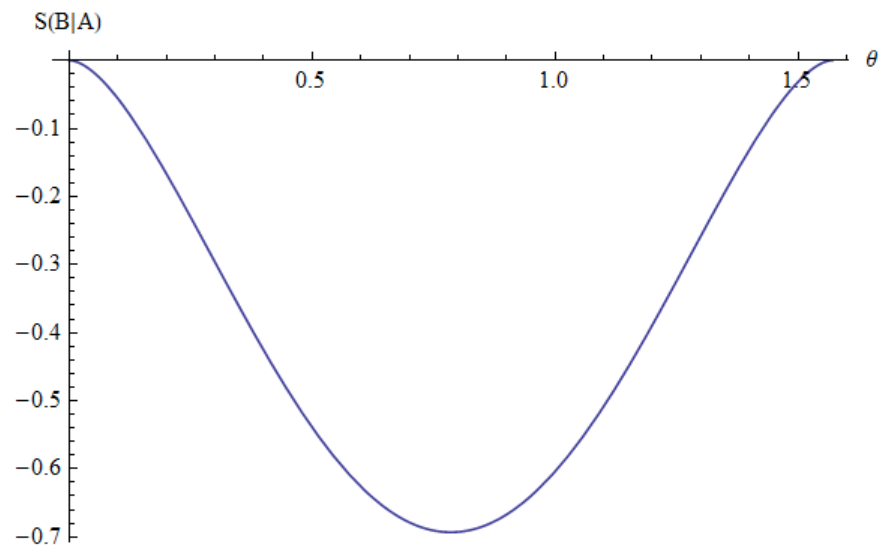
\includegraphics[scale=0.9]{figures/cond_ent_plot.png}
\caption{We can easily see that the minimum is close to $-\log2$. This is not an accident since is common among the so called maximally entangled states. In particular, $\theta= \pi /4$ will give the maximal entanglement \eqref{condentpsi}.}\label{figuraki6}
\end{center}
\end{figure}
\end{itemize}
